\chapter{Identification des activités et des tâches}

Nous allons, dans cette partie, identifier les activités et les tâches nécassaires à la réalisation des livrables attendus pour la phase d'étude préalable. A chaque tâche, correspondant pour la plupart à 2h de travail par semaine, sera ensuite affectée une ressource (des fois plusieurs). Les tâches seront enfin ordonnancées en fonction des échéances et des disponibilités des ressources. Nous considérons que la charge de travail par ressource est, en moyenne, de 5 heures par semaine.

\section{Liste des tâches et estimation des charges}

\begin{enumerate}
  \item Sous-phase d'initialisation
          \begin{enumerate}
            \item Organisation de l'étude :
              \begin{enumerate}
                  \item formaliser le cadre et le périmètre du projet (2h)
                  \item  recenser les objectifs, les contraintes et les risques de l'étude (2h)
                  \item  organiser l'équipe (distribution des rôles et des responsabilités) (2h)
                  \item  planifier la communication (30m)
                  \item  définir les livrables (1h)
              \end{enumerate}
            \item Planification de l'étude : 
              \begin{enumerate}
                  \item  découper en phases et sous-phases l'étude (1h)
                  \item  identifier les livrables intermédiaires (1h)
                  \item  définir les tâches (2h)
                  \item  évaluer les charges des tâches (2h)
                  \item  répartir et ordonnancer les tâches (2h)
              \end{enumerate}

            \item Planification des formations (30m):
                \begin{enumerate}
                  \item identifier et planifier les formations et leur affecter des ressources
                \end{enumerate}
            \item Choix techniques : 
                \begin{enumerate}
                  \item choisir les méthodes et les outils (2h)
                \end{enumerate}

            \item Prévention :
                \begin{enumerate}
                  \item diffuser le PAQ (2h)
                  \item définir le référenciel d'évaluation interne et externe (2h)
                  \item mettre en place un plan qualité (2h)
                \end{enumerate}

            \item Rédaction des livrables : 
                \begin{enumerate}
                  \item rédiger le dossier d'initialisation 
                  \item rédiger le PAQ 
                \end{enumerate}

            \item Contrôle :
              \begin{enumerate}
                \item revue des livrables (2h)
                \item réunion d'organisation et point sur le travail (1h) 
                \item rédaction des fiches de suivi et du tableau de bord (1h)
              \end{enumerate}
      \end{enumerate}

    \item Sous-phase d'expression des besoins
          \begin{enumerate}
            \item Formations 
                \begin{enumerate}
                  \item ARIS (1h)
                  \item SAP (1h)
                \end{enumerate}
            \item Définition du contexte et du périmètre de l'étude :
                \begin{enumerate}
                  \item décrire les sous-processus à analyser : (3h)
                    \begin{itemize}
                      \item offre et revue d'offre 
                      \item commandde et revue de commande
                      \item lancement des prestations de service et travaux
                      \item réalisation de prestations de maintenance
                      \item réalisation travaux induits
                      \item évolution du contrat
                      \item solde de l'affaire et du contrat 
                    \end{itemize}
                  \item modèles organisationnel, communicationnel, procédural (2h)
                  \item tableau croisé Services/Activités (2h) 
                \end{enumerate}
            \item Diagnostique du SI actuel du point de vue organisationnel : 
                \begin{enumerate}
                  \item décrire l'organisation actuelle du SI (rôles, responsabilités et activités réalisées) (2h)
                  \item représenter les processus et les procédures (2h)
                  \item identifier les dysfonctionnements et les écarts (2h)
                \end{enumerate}
            \item Diagnostique du SI actuel du point de vue informatique : 
                \begin{enumerate}
                  \item décrire l'architecture applicative (2h)
                  \item décrire l'architecture technique (2h)
                  \item cartographie applicative (2h)
                  \item cartographie technique (2h)
                  \item rédiger les fiches application (2h)
                  \item rédiger une synthèse des points forts et des points faibles (2h)
                \end{enumerate}
            \item Analyse des solutions des entreprises leader dans le domaine : 
                \begin{enumerate}
                  \item identifier les entreprises à analyser et pour quel domaine (2h)
                  \item étudier les progiciels de gestion intégrés (2h)
                  \item comprendre les méthodes et prendre connaîssance des indicateurs des entreprises identifiées (quantités, délais, coûts) (2h)
                  \item se situer par rapport aux progiciels (2h)
                  \item se situer par rapport aux performances des entreprises (2h)
                  \item capitaliser leurs meilleures pratiques (2h)
                \end{enumerate}
            \item Elaboration de la cible fonctionnelle : 
                \begin{enumerate}
                  \item créer les modèles de processus et d'activités (2h)
                  \item créer les modèles d'organisation type (2h)
                  \item créer les modèles généraux d'objets métiers à gérer (2h)
                  \item créer les diagrammes types de cas d'utilisation (2h)
                \end{enumerate}
            \item Identification des thèmes de progrès : 
                \begin{enumerate}
                  \item décliner la stratégie de l'entreprise au niveau des processus existants (2h)
                  \item adapter la logique des processus en s'appuyant sur l'architecture de référence (2h)
                  \item adapter l'organisation des acteurs impliqués en fonction des principes d'organisation de la référence (2h)
                  \item identifier les nouvelles technologies à forte valeur ajoutée (2h)
                \end{enumerate}
            \item Composition des livrables : 
                \begin{enumerate}
                  \item rapport de synthèse de l'étude de l'existant 
                  \item rapport de Benchmarking
                  \item rapport de modélisation de la cible fonctionnelle
                \end{enumerate}
            \item Contrôle :
              \begin{enumerate}
                \item revue des livrables (6h)
                \item réunion d'organisation et point sur le travail (3h) 
                \item rédaction des fiches de suivi et du tableau de bord (3h)
              \end{enumerate}
      \end{enumerate}

    \item Sous-phase de construction des solutions

          \begin{enumerate}
            \item Description des impacts sur l'organisation : 
                \begin{enumerate}
                  \item identifier les changements organisationnels (2h)
                  \item mesurer les risques induits des changements des solutions :
                    \begin{itemize}
                      \item standard (1h)
                      \item spécifique (1h)
                    \end{itemize}
                  \item dimensionner les actions à conduire dans les étapes ultérieures pour la solution :
                    \begin{itemize}
                      \item standard (1h)
                      \item spécifique (1h)
                    \end{itemize}
                \end{enumerate}
            \item Analyse de l'architecture applicative cible : 
                \begin{enumerate}
                  \item identifier les paquetages et les classes importantes de l'analyse et les exigences particulières à satisfaire (2h)
                  \item identifier les échanges entre paquetages et les interfaces disponibles (2h)
                \end{enumerate}
            \item Définition des stratégies d'informatisation : 
                \begin{enumerate}
                  \item rechercher les hypothèses envisageables (6h)
                  \item prioriser les hypothèses identifiées (2h)
                  \item concevoir et dimensionner les parties du système, l'architecture logique d'ensemble et l'architecture technique pour la première hypothèse (2h)
                  \item concevoir et dimensionner les parties du système, l'architecture logique d'ensemble et l'architecture technique pour la deuxième hypothèse (2h)
                \end{enumerate}
            \item Conception architecturale logique et technique : 
                \begin{enumerate}
                  \item identifier les solutions progiciel candidates (6h)
                  \item analyser les écarts fonctionnels avec les besoins utilisateurs (2h)  
                  \item identifier les solutions pour traiter les écarts fonctionnels (2h)
                  \item faire un mapping sur l'architecture applicative cible (2h)
                \end{enumerate}
            \item Composition des livrables : 
                \begin{enumerate}
                  \item rédiger le rapport de spécification d'une solution spécifique (8h)
                  \item rédiger le rapport de configuration des scénarii SAP sélectionnés (4h)
                  \item créer les matrices ARIS SAP / fonction SPIE SE et SAP / organigramme SPIE SE (3h)
                  \item générer grâce à ARIS le rapport de modélisation de la solution sélecionnée (30min)
                \end{enumerate}
            \item Contrôle :
              \begin{enumerate}
                \item revue des livrables (4h)
                \item réunion d'organisation et point sur le travail (2h) 
                \item rédaction des fiches de suivi et du tableau de bord (2h)
              \end{enumerate}
      \end{enumerate}

    \item Sous-phase d'élaboration, évaluation et choix des scénarii

          \begin{enumerate}
            \item Identification des scénarii de mise en oeuvre :
                \begin{enumerate}
                  \item créer un scénario pour la solution standard (2h)
                  \item créer un scénario pour la solution spécifique (2h)
                  \item planifier la mise en oeuvre de la solution standard (2h)
                  \item planifier la mise en oeuvre de la solution spécifique (2h)
                \end{enumerate}
            \item Composition des livrables :
                \begin{enumerate}
                  \item rédiger le dossier de choix pour le Comité de Pilotage (6h)
                \end{enumerate}
            \item Contrôle :
              \begin{enumerate}
                \item revue des livrables (2h)
                \item réunion d'organisation et point sur le travail (1h) 
                \item rédaction des fiches de suivi et du tableau de bord (1h)
              \end{enumerate}
      \end{enumerate}

    \item Sous-phase de bilan

          \begin{enumerate}
            \item Préparation des bilans qualitatif et quantitatif :
                \begin{enumerate}
                  \item comparer le contenu du dossier d'initialisation et les livrables effectivement rendus (2h)
                  \item estimer les charges effectives et expliquer les eventuelles différences avec le plan de charge (2h)
                  \item faire un bilan humaine du travail de l'équipe et de ses membres (2h)
                \end{enumerate}
            \item Composition des livrables :
                \begin{enumerate}
                  \item rédiger le dossier de bilan (4h)
                  \item préparer une présentation powerpoint du projet (8h)
                \end{enumerate}
            \item Contrôle :
              \begin{enumerate}
                \item revue des livrables (2h)
                \item réunion d'organisation et point sur le travail (1h) 
                \item rédaction des fiches de suivi et du tableau de bord (1h)
              \end{enumerate}
          \end{enumerate}

\end{enumerate}

\section{Diagramme de GANTT (version 0)}

\begin{figure}[h]
    \centering
    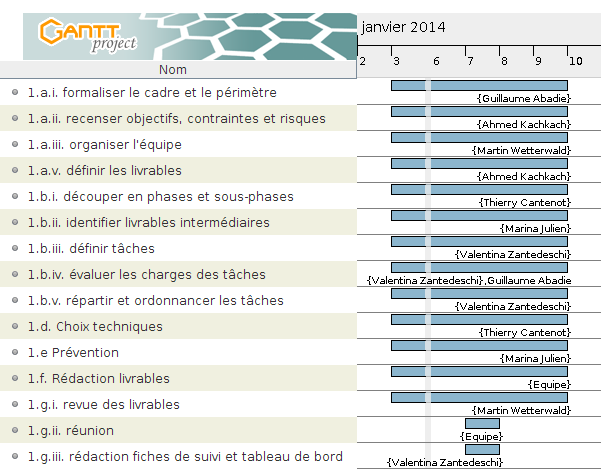
\includegraphics[scale=0.8]{images/Gantt_1.png}
    \caption{Sous-phase d'initialisation}
    \label{diagram:si_map}
\end{figure}

\begin{figure}[h]
    \centering
    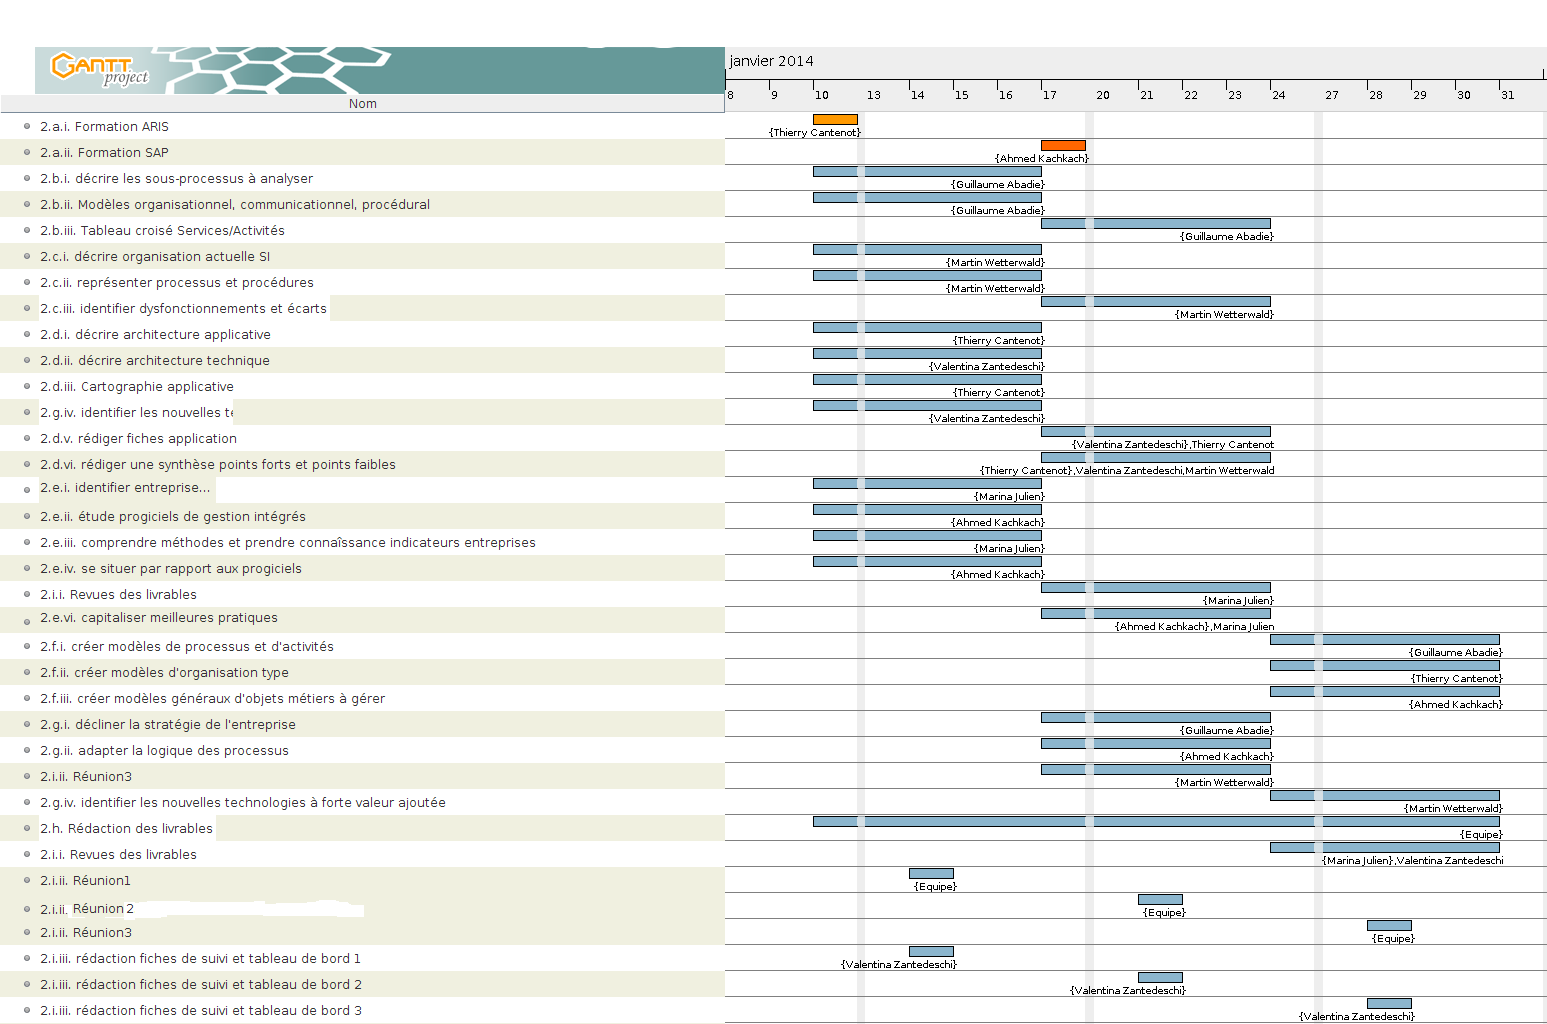
\includegraphics[width=150mm]{images/Gantt_2.png}
    \caption{Sous-phase d'expression des besoins}
    \label{diagram:si_map}
\end{figure}

\begin{figure}[h]
    \centering
    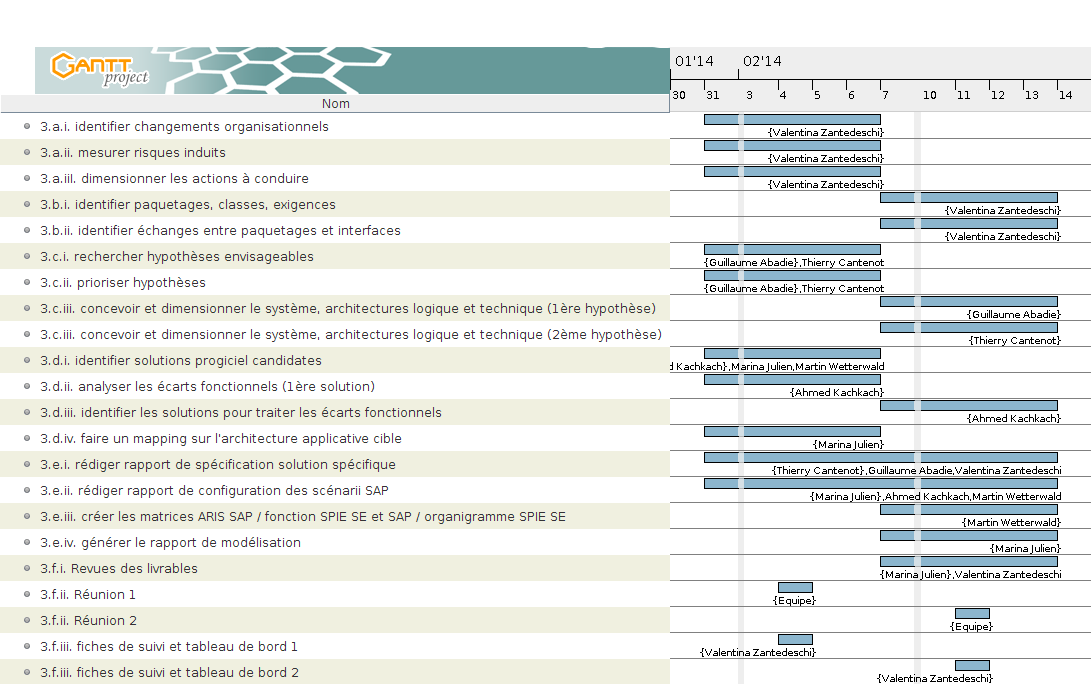
\includegraphics[width=150mm]{images/Gantt_3.png}
    \caption{Sous-phase de construction des solutions}
    \label{diagram:si_map}
\end{figure}

\begin{figure}[h]
    \centering
    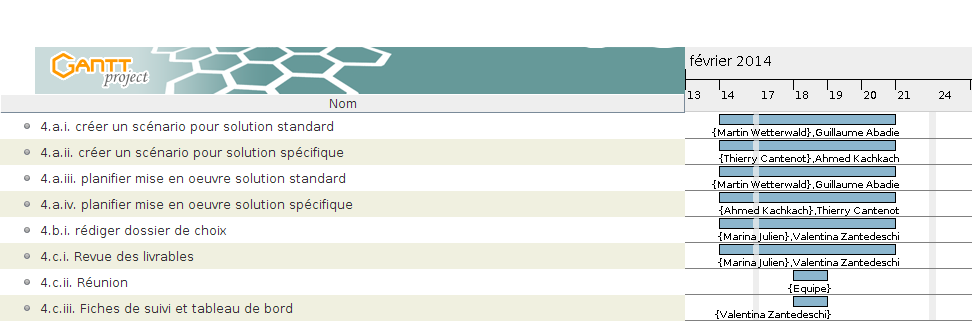
\includegraphics[scale=0.65]{images/Gantt_4.png}
    \caption{Sous-phase d'élaboration, évaluation et choix des scénarii}
    \label{diagram:si_map}
\end{figure}

\begin{figure}[h]
    \centering
    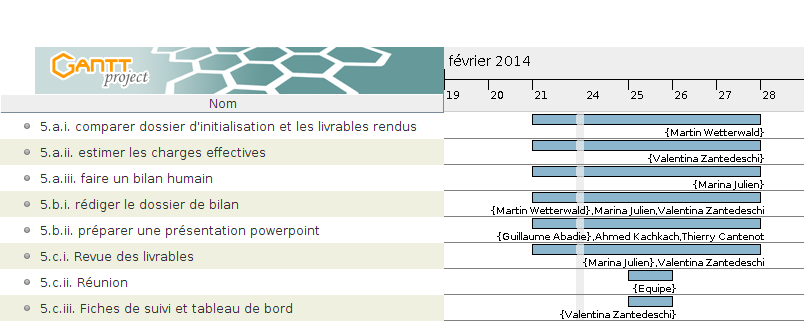
\includegraphics[scale=0.6]{images/Gantt_5.png}
    \caption{Sous-phase de bilan}
    \label{diagram:si_map}
\end{figure}
